% 2.4
\section{順序項木パターン}
\textbf{順序木(ordered tree)}とは,同じ親を持つ頂点に順序関係(兄弟関係)を持つ木のことである.順序木の例を図\ref{fig:sibling_relationship}に示す.これらの木は異なる木として扱われる.

% 定義6
\begin{define}{\bf 順序木における変数}\par
  $\ell$を1以上の整数とする.$T=(V_T,E_T)$を順序木とする.順序木$T$の変数とは,次の条件(1)--(3)を満たす$V_T$に含まれる頂点のリスト$h=[v_0,v_1,\ldots,v_{\ell}]$である.
  \begin{enumerate}
    \item[(1)] 頂点$v_0$は子を持つ.
    \item[(2)] $v_1,v_2,\ldots,v_{\ell}$ $(v_i \in V_T, 1\leq i\leq \ell)$は$v_0$の連続した子である.
    \item[(3)] 変数$h$にはランクが$\ell+1$の変数ラベル$x\in X$がラベル付けされている.
  \end{enumerate}
  無順序木における変数と同様に,$v_0$を変数$h$の親ポート,$v_1,v_2,\ldots,v_{\ell}$を変数$h$の子ポートと呼び,変数$h=[v_0,v_1,\ldots,v_{\ell}]$の次元を$\ell+1$とする.
\end{define}

% 定義7
\begin{define}{\bf 順序項木パターン(ordered term tree pattern)}\par
$T=(V_T,E_T)$を順序木とし,$H_T$を$T$の変数の集合とする.ただし,任意の異なる2つの変数$h_1,\,h_2\in H_T$に対して,$h_1$と$h_2$に共通して現れる頂点は高々1つであるとする.順序項木パターンとは,次の条件(1)--(4)を満たす3つ組$t=(V_t,E_t,H_t)$である:
\begin{enumerate}
  \item[(1)] $V_t=V_T$,
  \item[(2)] $E_t=E_T\setminus \left(\bigcup_{[v_0,v_1,\ldots,v_{\ell}]\in H_T}\{(v_0,v_i)\in E_T\mid 1\leq i\leq \ell\}\right)$,
  \item[(3)] $H_t=H_T$,
  \item[(4)] $V_t$に属す頂点の頂点ラベル,$E_t$に属す辺の辺ラベルは,それぞれに対応する$V_T$の頂点ラベル,$E_T$の辺ラベルと同じである.
\end{enumerate}
\end{define}

% 定義8
\begin{define}{\bf 順序項木パターンの束縛と代入}\par
  $x\in X$をランク$\ell+1$の変数ラベル,$g$を$\ell+1$個以上の頂点を持つ順序項木パターンとする.また,$u_0$を$g$の根とし,$u_1,\ldots,u_{\ell}$を$g$の根以外の互いに異なる$\ell$個の葉で,$u_i$が$u_{i+1}$ $(1\leq i\leq \ell-1)$より左の葉であるとき,$\sigma=[u_0,u_1,\ldots,u_{\ell}]$とする.このとき,形式$x:=[g,\sigma]$を$x$の\textbf{束縛(binding)}という.
  $f=(V_{f},E_{f},H_{f})$を順序項木パターンとする.ランク$\ell+1$の変数ラベル$x$を持つ変数が$f$に存在するとき,その変数を$h_1,\ldots,h_k$ $(k\geq 0)$とする.束縛$x:=[g,\sigma]$を変数$h_1,\ldots,h_k$に次のように同時に適用して得られる順序項木パターンを$f\{x:=[g,\sigma]\}$と書く:
  \begin{enumerate}
    \item[(1)] $g_1,\ldots,g_k$を順序項木パターン$g$と同型な順序項木パターンとする.
    \item[(2)] 変数$h_j=[v_0^{(j)},v_1^{(j)},\ldots,v_{\ell}^{(j)}]$ $(1\leq j\leq k)$に関して,$H_f$から変数$h_j$を削除し,$g$の頂点$u_0,u_1,\ldots,u_{\ell}$に対応する$g_j$の頂点$u_0^{(j)},u_1^{(j)},\ldots,u_{\ell}^{(j)}$を,この順序で変数$h_j$の頂点$v_0^{(j)},v_1^{(j)},\ldots,v_{\ell}^{(j)}$と同一視する.同一視後の頂点ラベルは,頂点$v_0^{(j)},v_1^{(j)},\ldots,v_{\ell}^{(j)}$の頂点ラベルを継承する.
  \end{enumerate}
  束縛による兄弟関係は,$f$と$g$の兄弟関係を拡張して定める\cite{suzuki-tcs2006}.
  \textbf{代入(substitution)}とは,$x_i\,(1\leq i\leq n)$が$X$の異なる変数ラベルであるような束縛の有限集合$\theta=\{x_1:=[g_1,\sigma_1],\ldots,x_n:=[g_n,\sigma_n]\}$である.
  ただし,$g_{1},\ldots,g_{n}$には変数ラベル$x_1,\ldots,x_n$を持つ変数が現れないと仮定する.
  代入$\theta$による$f$の\textbf{インスタンス(instance)}とは,$f$に対して,$\theta$の全ての束縛$x_i:=[g_i,\sigma_i]$ $(1\leq i\leq n)$を適用して得られる順序項木パターンである.代入$\theta$による$f$のインスタンスを$f\theta$と書く.

  $\Sigma,\Lambda$を頂点ラベルの集合,辺ラベルの集合とする順序木の全体を${\cal OT}_{\Sigma,\Lambda}$とする.また,$\Sigma,\Lambda,X$を頂点ラベルの集合,辺ラベルの集合,変数ラベルの集合とする順序項木パターンの全体を${\cal OTTP}_{\Sigma,\Lambda,X}$とする.次のように${\cal OTTP}_{\Sigma,\Lambda,X}$の部分集合を定める:
  \begin{eqnarray*}
  {\cal LOTTP}_{\Sigma,\Lambda,X} & = & \{t=(V_t,E_t,H_t)\in{\cal OTTP}_{\Sigma,\Lambda,X}\mid\\
  & & \hspace*{12pt}\forall h_1,\,h_2\in H_t\,(h_1\not= h_2)\mbox{に対して,$h_1$と$h_2$の変数ラベルは異なる}\}
  \end{eqnarray*}

  \noindent
  ${\cal LOTTP}_{\Sigma,\Lambda,X}$に属す順序項木パターンを\textbf{線形順序項木パターン(linear ordered term tree pattern)}と呼ぶ.

  以降,順序木$T=(V_T,E_T)$を,変数を持たない順序項木パターン$T=(V_T,E_T,\emptyset)$とみなす.
\end{define}

% 図2.5
\begin{figure}[tb]
  \centering
  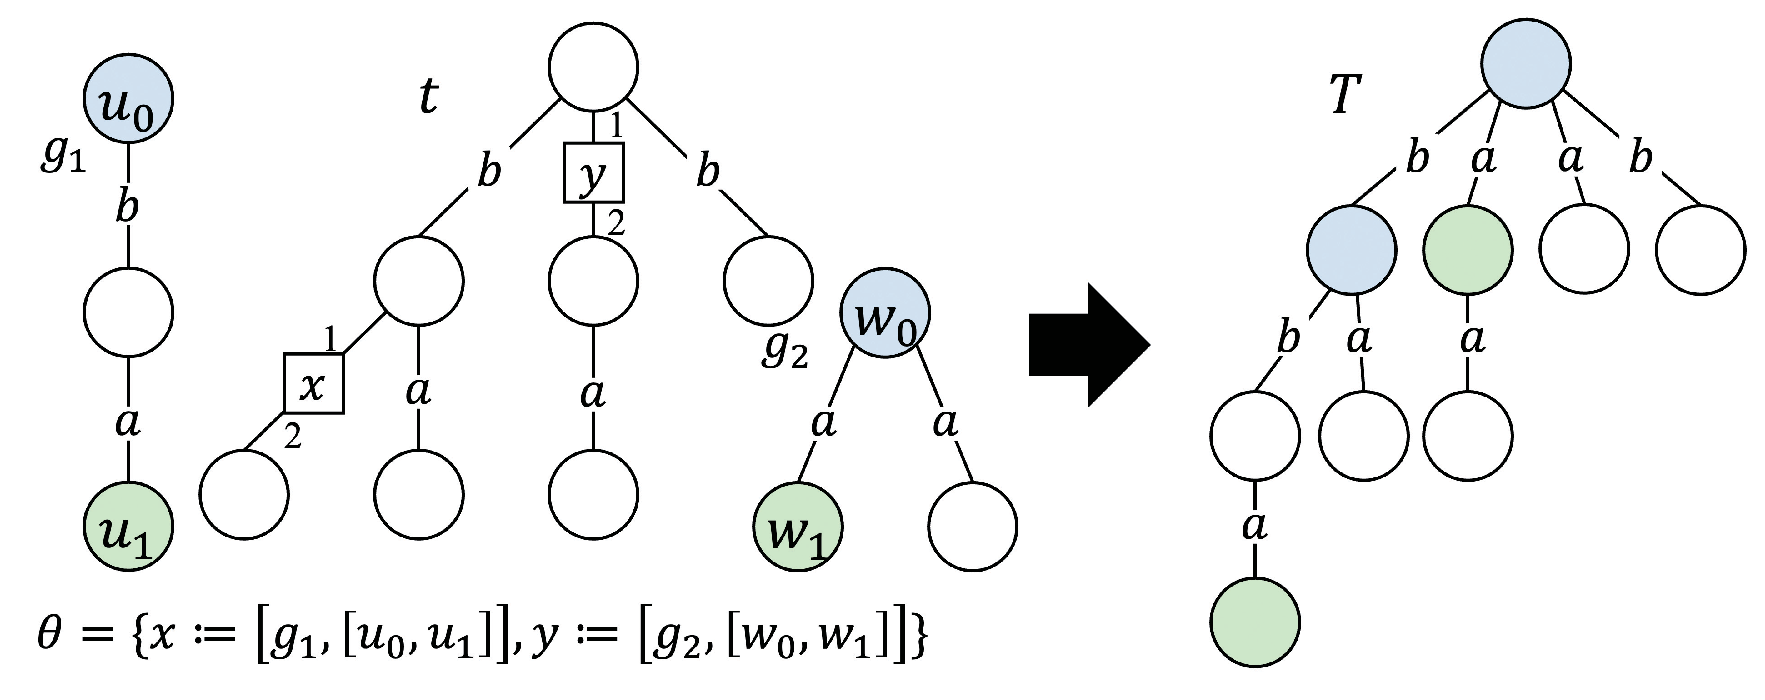
\includegraphics[scale=0.5]{fig-lottp.eps}
  \caption{線形順序項木パターン$t$と順序木$t\theta \equiv T$}\label{fig:lottp}
\end{figure}

% 定義9
\begin{define}{\bf 順序項木パターン言語}\par
  順序項木パターン$t\in {\cal OTTP}_{\Sigma,\Lambda,X}$に対して,$t$の順序項木パターン言語$L(t)\subseteq {\cal OT}_{\Sigma,\Lambda}$を次のように定義する:
  $$L(t)=\{t\theta\in {\cal OT}_{\Sigma,\Lambda}\mid \mbox{$\theta$は$t$の変数への任意の代入}\}.$$

  \noindent
  順序項木パターン$t$に対して,$T\in L(t)$となる順序木$T$の例を図\ref{fig:lottp}にあげる.
\end{define}

線形順序項木パターン$t$と順序木$T$に対して,$t\theta\equiv T$となるような代入$\theta$が存在するとき,$t$は$T$にマッチするという.線形順序項木パターン照合問題は次のように定義される決定問題である:

\medskip
\noindent
\textbf{線形順序項木パターン照合問題}(${\cal LOTTP}$-${\cal MP}$)\\
\textbf{入力}: 線形順序項木パターン$t$と順序木$T$.\\
\textbf{問題}: $t$は$T$にマッチするか?
\medskip

Suzuki et al.\cite{suzuki-tcs2006}は,線形順序項木パターン照合問題を解く$O(nN)$時間逐次アルゴリズムを提案した.$n$と$N$はそれぞれ線形順序項木パターン及び順序木の頂点数である.